\chapter{Proposta de Solução}

Este capítulo apresenta a proposta de solução para o problema investigado, descrevendo a documentação técnica inicial do sistema, os requisitos identificados, os principais artefatos de modelagem e a visão geral do protótipo.

\section{Documentação Técnica}

A documentação técnica da solução tem como objetivo organizar, de forma estruturada, as decisões relacionadas ao funcionamento do sistema, às integrações previstas e ao comportamento esperado da aplicação. Nesta etapa, a documentação cumpre o papel de consolidar os resultados da pesquisa com usuários e transformá-los em especificações iniciais para desenvolvimento.

\subsection{Levantamento de Requisitos}

O levantamento de requisitos foi orientado pelos achados da pesquisa qualitativa e pelas histórias de usuário definidas no capítulo anterior. A seguir, são apresentados requisitos iniciais que servirão de base para o detalhamento técnico da solução.

\subsubsection{Requisitos Funcionais}

\begin{itemize}
    \item O sistema deve interpretar e processar mensagens enviadas pelo usuário via WhatsApp utilizando Inteligência Artificial.
    \item O sistema deve identificar automaticamente os valores, tipos de movimentação (receita/despesa) e categorias presentes nas mensagens de linguagem natural do usuário.
    \item O sistema deve gerar gráficos financeiros com base nos dados registrados pelo usuário.
    \item O sistema deve permitir que o usuário possa se cadastrar.
    \item O sistema deve permitir que o usuário faça o login, baseado nos dados cadastrados.
    \item O sistema deve ter uma visualização web, que permita ao usuário ver os dashboards criados.
    \item O sistema deve permitir separar gastos por categorias.
    \item O sistema deve permitir a configuração do estilo de comunicação do assistente virtual conforme a preferência do usuário.
    \item O sistema deve permitir que o usuário reserve valores para metas financeiras específicas, desconsiderando-os do saldo disponível.
    \item O sistema deve permitir que o usuário edite as movimentações financeiras registradas.
    \item O sistema deve permitir que o usuário remova as movimentações financeiras registradas.
    \item O sistema deve permitir a geração de relatórios financeiros com base nos dados registrados pelo usuário.
    \item O sistema deve permitir que o usuário exporte o relatório para fora do site.
    \item O assistente de IA deve manter o contexto da conversa com o usuário, permitindo interações contínuas e mais fluidas.
\end{itemize}

\subsubsection{Requisitos Não Funcionais}

\begin{itemize}
    \item O sistema deve apresentar fluxo de uso simples, intuitivo e compatível com usuários sem conhecimento técnico.
    \item O processo de registro financeiro deve exigir o menor número de etapas, reduzindo o esforço necessário para utilização contínua da plataforma.
    \item A interface conversacional deve utilizar linguagem clara, objetiva e de fácil compreensão para o usuário.
    \item O sistema deve permitir utilização em dispositivos móveis, considerando que o WhatsApp será o principal canal de interação.
    \item O sistema deve garantir persistência, integridade e segurança dos dados financeiros registrados pelos usuários.
    \item A solução deve possuir arquitetura modular, permitindo evolução futura das integrações e funcionalidades.
    \item A aplicação deve ser coerente com execução em ambiente conteinerizado utilizando Docker.
    \item O dashboard web deve apresentar informações financeiras de forma visual, organizada e acessível.
    \item O sistema deve priorizar facilidade de uso e baixo esforço mental, buscando incentivar constância no acompanhamento financeiro.
    \item O sistema deve oferecer experiência coerente com a rotina do dia a dia do usuário, permitindo registros rápidos por linguagem natural.
\end{itemize}

\subsection{Modelagem}

A modelagem do sistema possui papel fundamental no processo de desenvolvimento de software, pois permite representar de forma visual a estrutura, os componentes e os relacionamentos existentes na aplicação antes de sua implementação. Por meio da modelagem, torna-se possível compreender melhor o funcionamento do sistema, organizar os requisitos levantados e facilitar a comunicação entre os integrantes do projeto. Além disso, os modelos desenvolvidos auxiliam na documentação da aplicação, contribuindo para o planejamento da arquitetura do software e para a definição das regras de negócio envolvidas no sistema.

No contexto da presente proposta, a modelagem foi utilizada para representar os principais elementos, para isso, foram elaborados diagramas voltados à representação estrutural e organizacional da aplicação, permitindo visualizar os componentes principais. Dessa forma, a modelagem contribui para demonstrar como os elementos do sistema se relacionam, além de servir como apoio para o desenvolvimento da solução proposta.

\subsubsection{Diagrama de Casos de Uso}

O diagrama de casos de uso consiste em uma representação da UML utilizada para apresentar, de maneira visual, as principais funcionalidades oferecidas por um sistema e as interações estabelecidas entre essas funcionalidades e seus atores. Os atores correspondem a usuários, sistemas externos ou outras entidades que se relacionam com o sistema, enquanto os casos de uso representam ações, processos ou objetivos que podem ser executados. Esse tipo de diagrama assume papel relevante nas etapas de levantamento e modelagem de requisitos, uma vez que contribui para a delimitação do escopo do sistema, para a identificação de suas funcionalidades centrais e para a facilitação da comunicação entre desenvolvedores, orientadores e demais envolvidos no projeto.

No diagrama de casos de uso desenvolvido para a proposta deste trabalho, o ator principal é o Usuário, responsável por interagir com o sistema para registrar transações financeiras por meio do WhatsApp, consultar saldo, acessar relatórios financeiros, cadastrar e acompanhar metas, visualizar o dashboard web e receber alertas financeiros. O diagrama também contempla funcionalidades internas necessárias ao funcionamento da solução, tais como interpretar linguagem natural, classificar transações, confirmar registros financeiros, identificar gastos recorrentes, gerar recomendações personalizadas, emitir relatórios e armazenar dados financeiros.

\begin{figure}[H]
    \centering
    \caption{Diagrama de casos de uso da solução proposta}
    \label{fig:diagrama-casos-uso}
    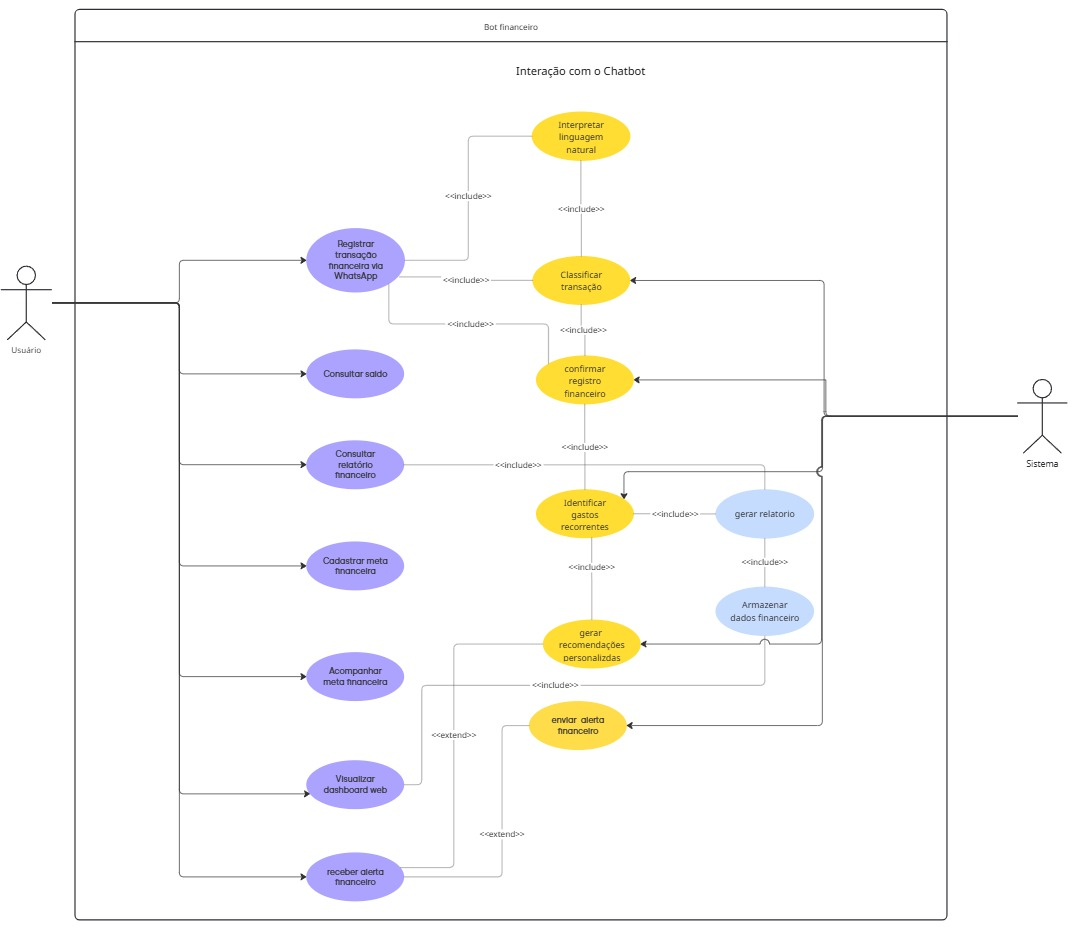
\includegraphics[width=\textwidth]{figs/diagrama-caso-de-uso.png}
    \fonte{Elaborado pelos autores.}
\end{figure}

\subsubsection{Diagrama de Classes}

O diagrama de classes é um dos diagramas mais utilizados da UML, sendo responsável por representar a estrutura estática de um sistema orientado a objetos. Esse tipo de diagrama permite demonstrar as classes existentes no sistema, seus atributos, métodos e os relacionamentos entre elas. Além disso, o diagrama de classes auxilia na visualização da organização do software, contribuindo para a compreensão da arquitetura do sistema e das responsabilidades de cada componente.

No contexto da presente proposta, o diagrama de classes contempla as entidades centrais pelo gerenciamento de usuários, mensagens, transações financeiras, categorias, metas financeiras e notificações. Além disso, o diagrama também apresenta uma classe de serviço responsável pelas funcionalidades de inteligência artificial, incluindo processamento de mensagens, geração de recomendações e emissão de alertas financeiros. Os relacionamentos apresentados demonstram como os componentes do sistema se conectam, permitindo a integração entre o controle financeiro, a comunicação conversacional e os recursos inteligentes propostos pela aplicação.

\begin{figure}[H]
    \centering
    \caption{Diagrama de classes}
    \label{fig:diagrama-classes}
    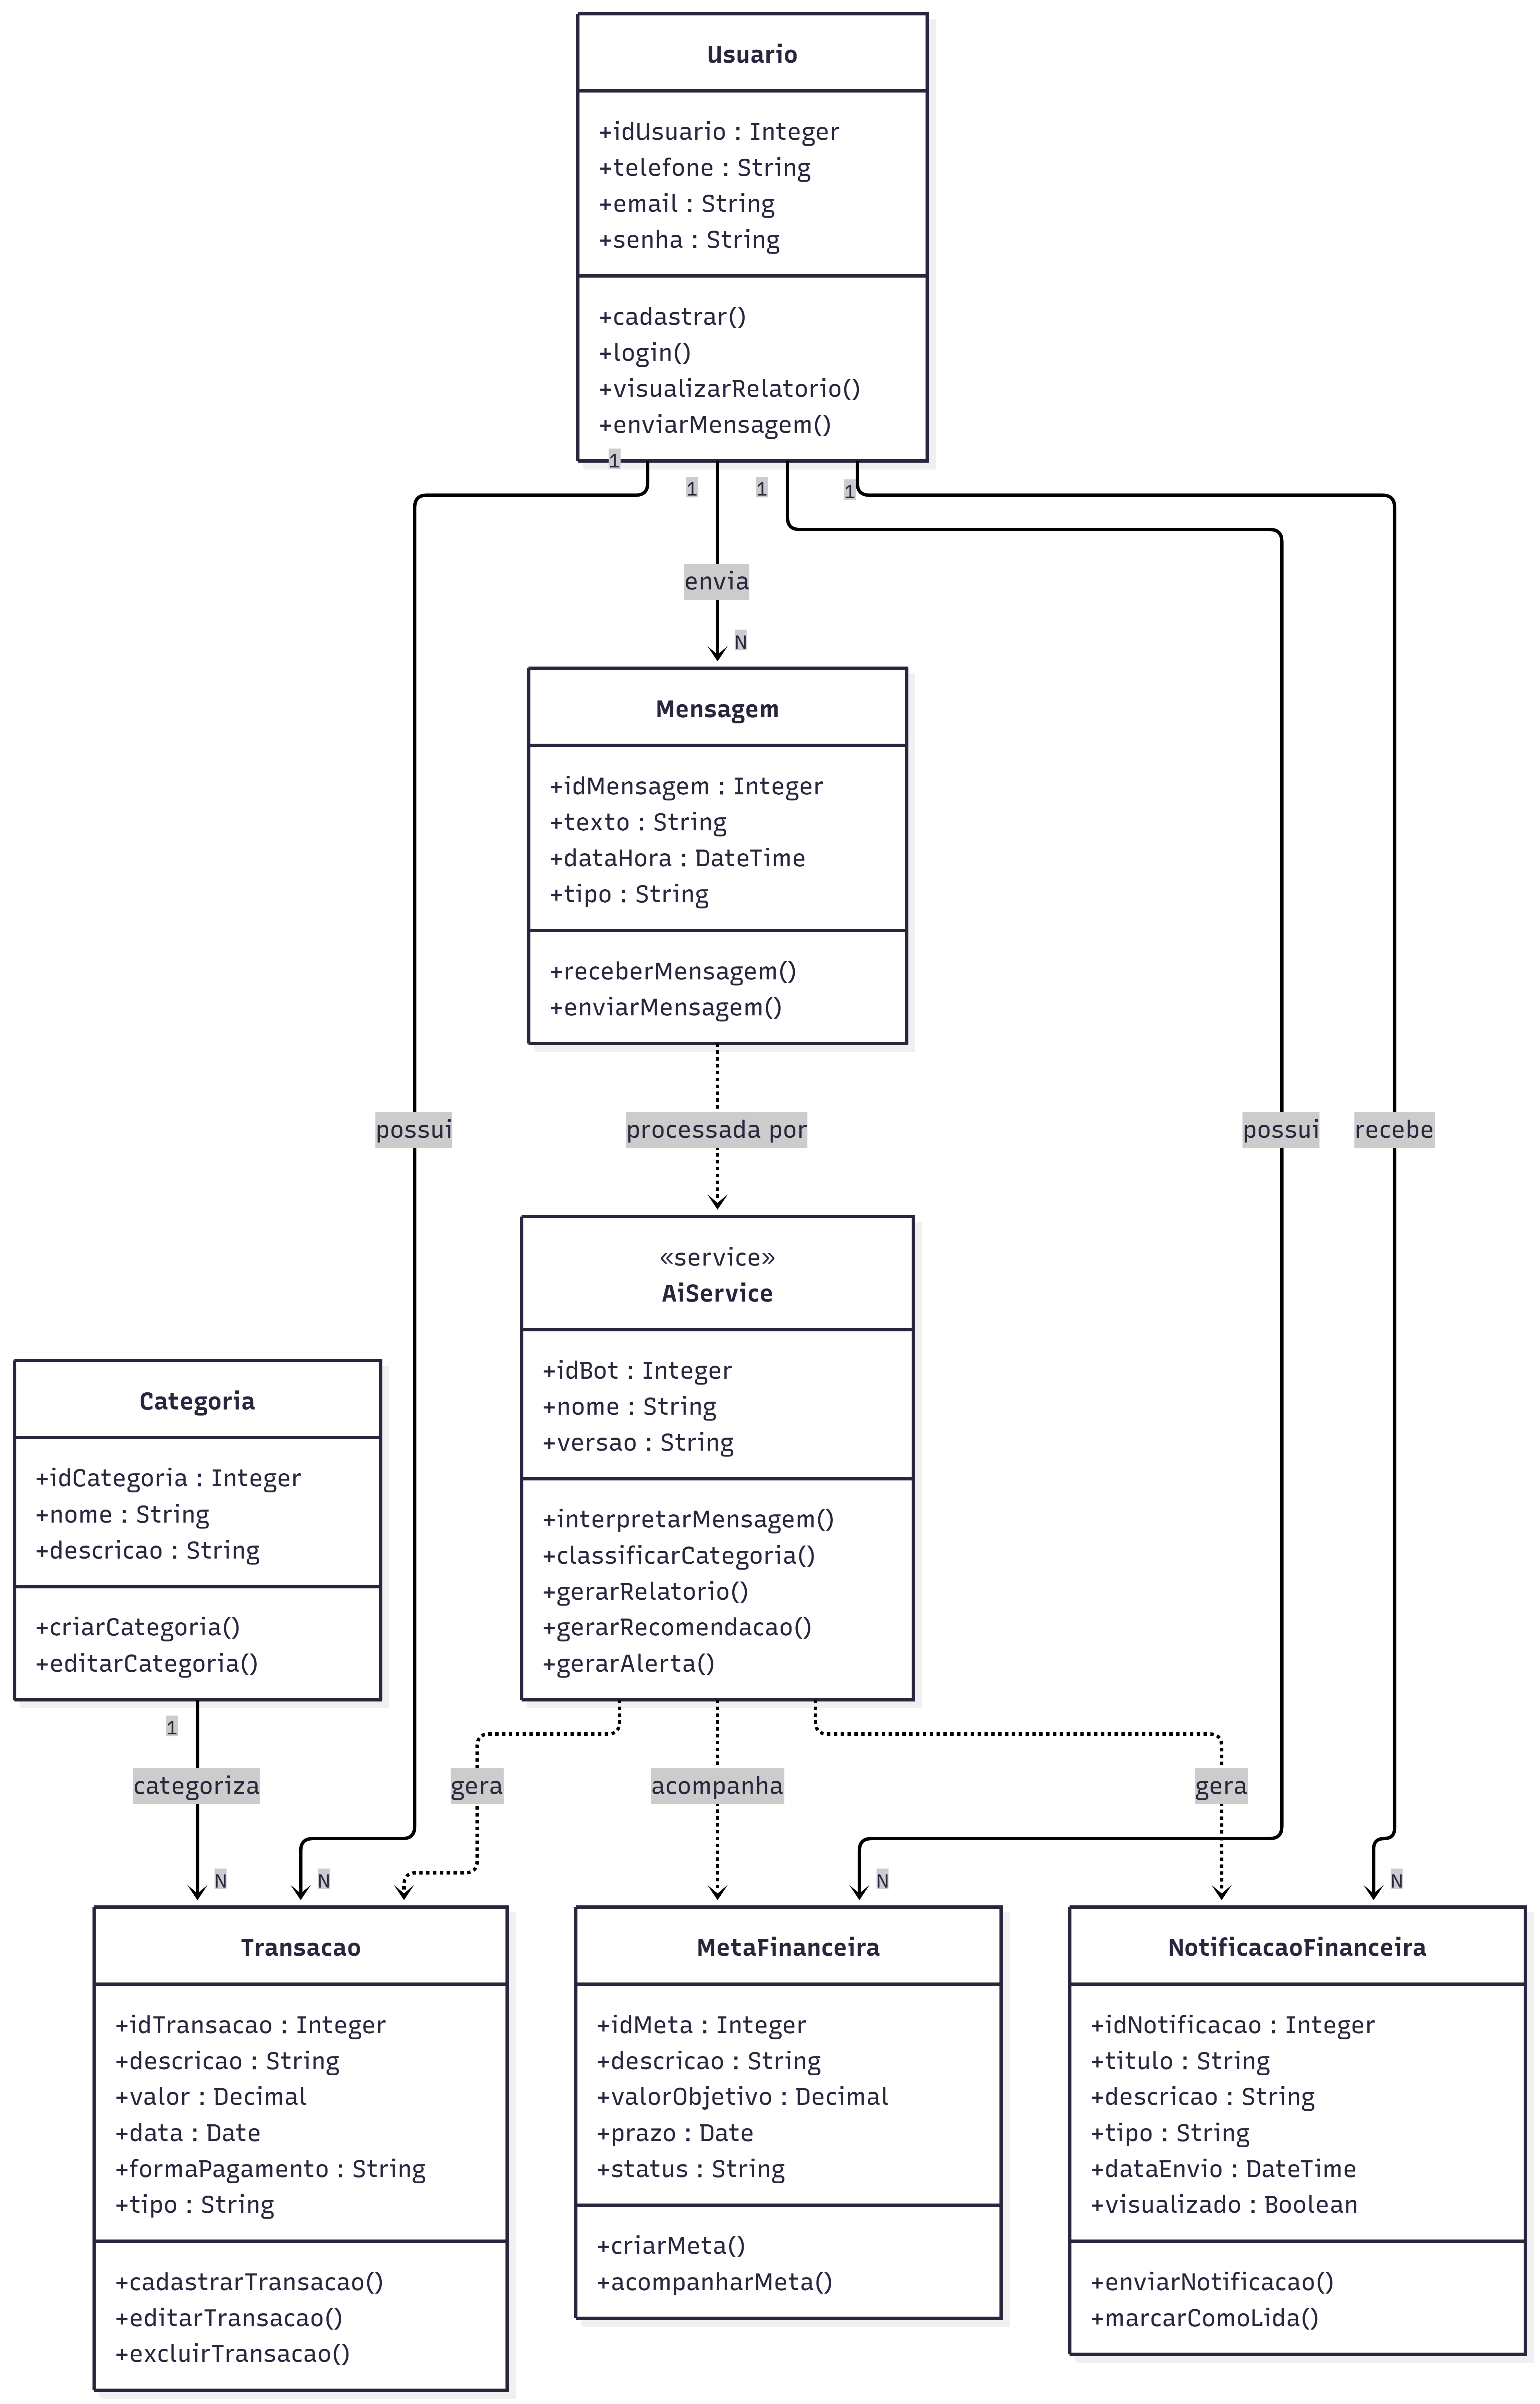
\includegraphics[width=0.8\textwidth]{figs/diagrama-de-classe.png}
    \fonte{Elaborado pelos autores.}
\end{figure}

\subsubsection{Diagrama Entidade-Relacionamento}

O diagrama entidade-relacionamento é uma técnica de modelagem utilizada para representar a estrutura lógica de um banco de dados, permitindo visualizar entidades, atributos e os relacionamentos existentes entre os dados do sistema. Esse tipo de diagrama auxilia na organização e no planejamento do banco de dados, contribuindo para a definição das informações que serão armazenadas e da forma como essas informações se relacionam dentro da aplicação. Além disso, o modelo entidade-relacionamento é amplamente utilizado durante o desenvolvimento de sistemas para facilitar a compreensão da estrutura dos dados e apoiar a implementação do banco de dados.

No contexto da presente proposta, o diagrama entidade-relacionamento representa as principais entidades relacionadas ao gerenciamento financeiro e à comunicação conversacional do sistema. A estrutura contempla entidades responsáveis pelo armazenamento de usuários, conversas, mensagens, transações financeiras, categorias, metas financeiras e notificações. Os relacionamentos apresentados demonstram como essas entidades se conectam dentro do banco de dados, permitindo o gerenciamento das informações financeiras, o armazenamento do histórico de conversas e o envio de notificações ao usuário. Dessa forma, o diagrama evidencia a organização dos dados necessários para o funcionamento da aplicação proposta.

\begin{figure}[H]
    \centering
    \caption{Diagrama entidade-relacionamento}
    \label{fig:diagrama-erd}
    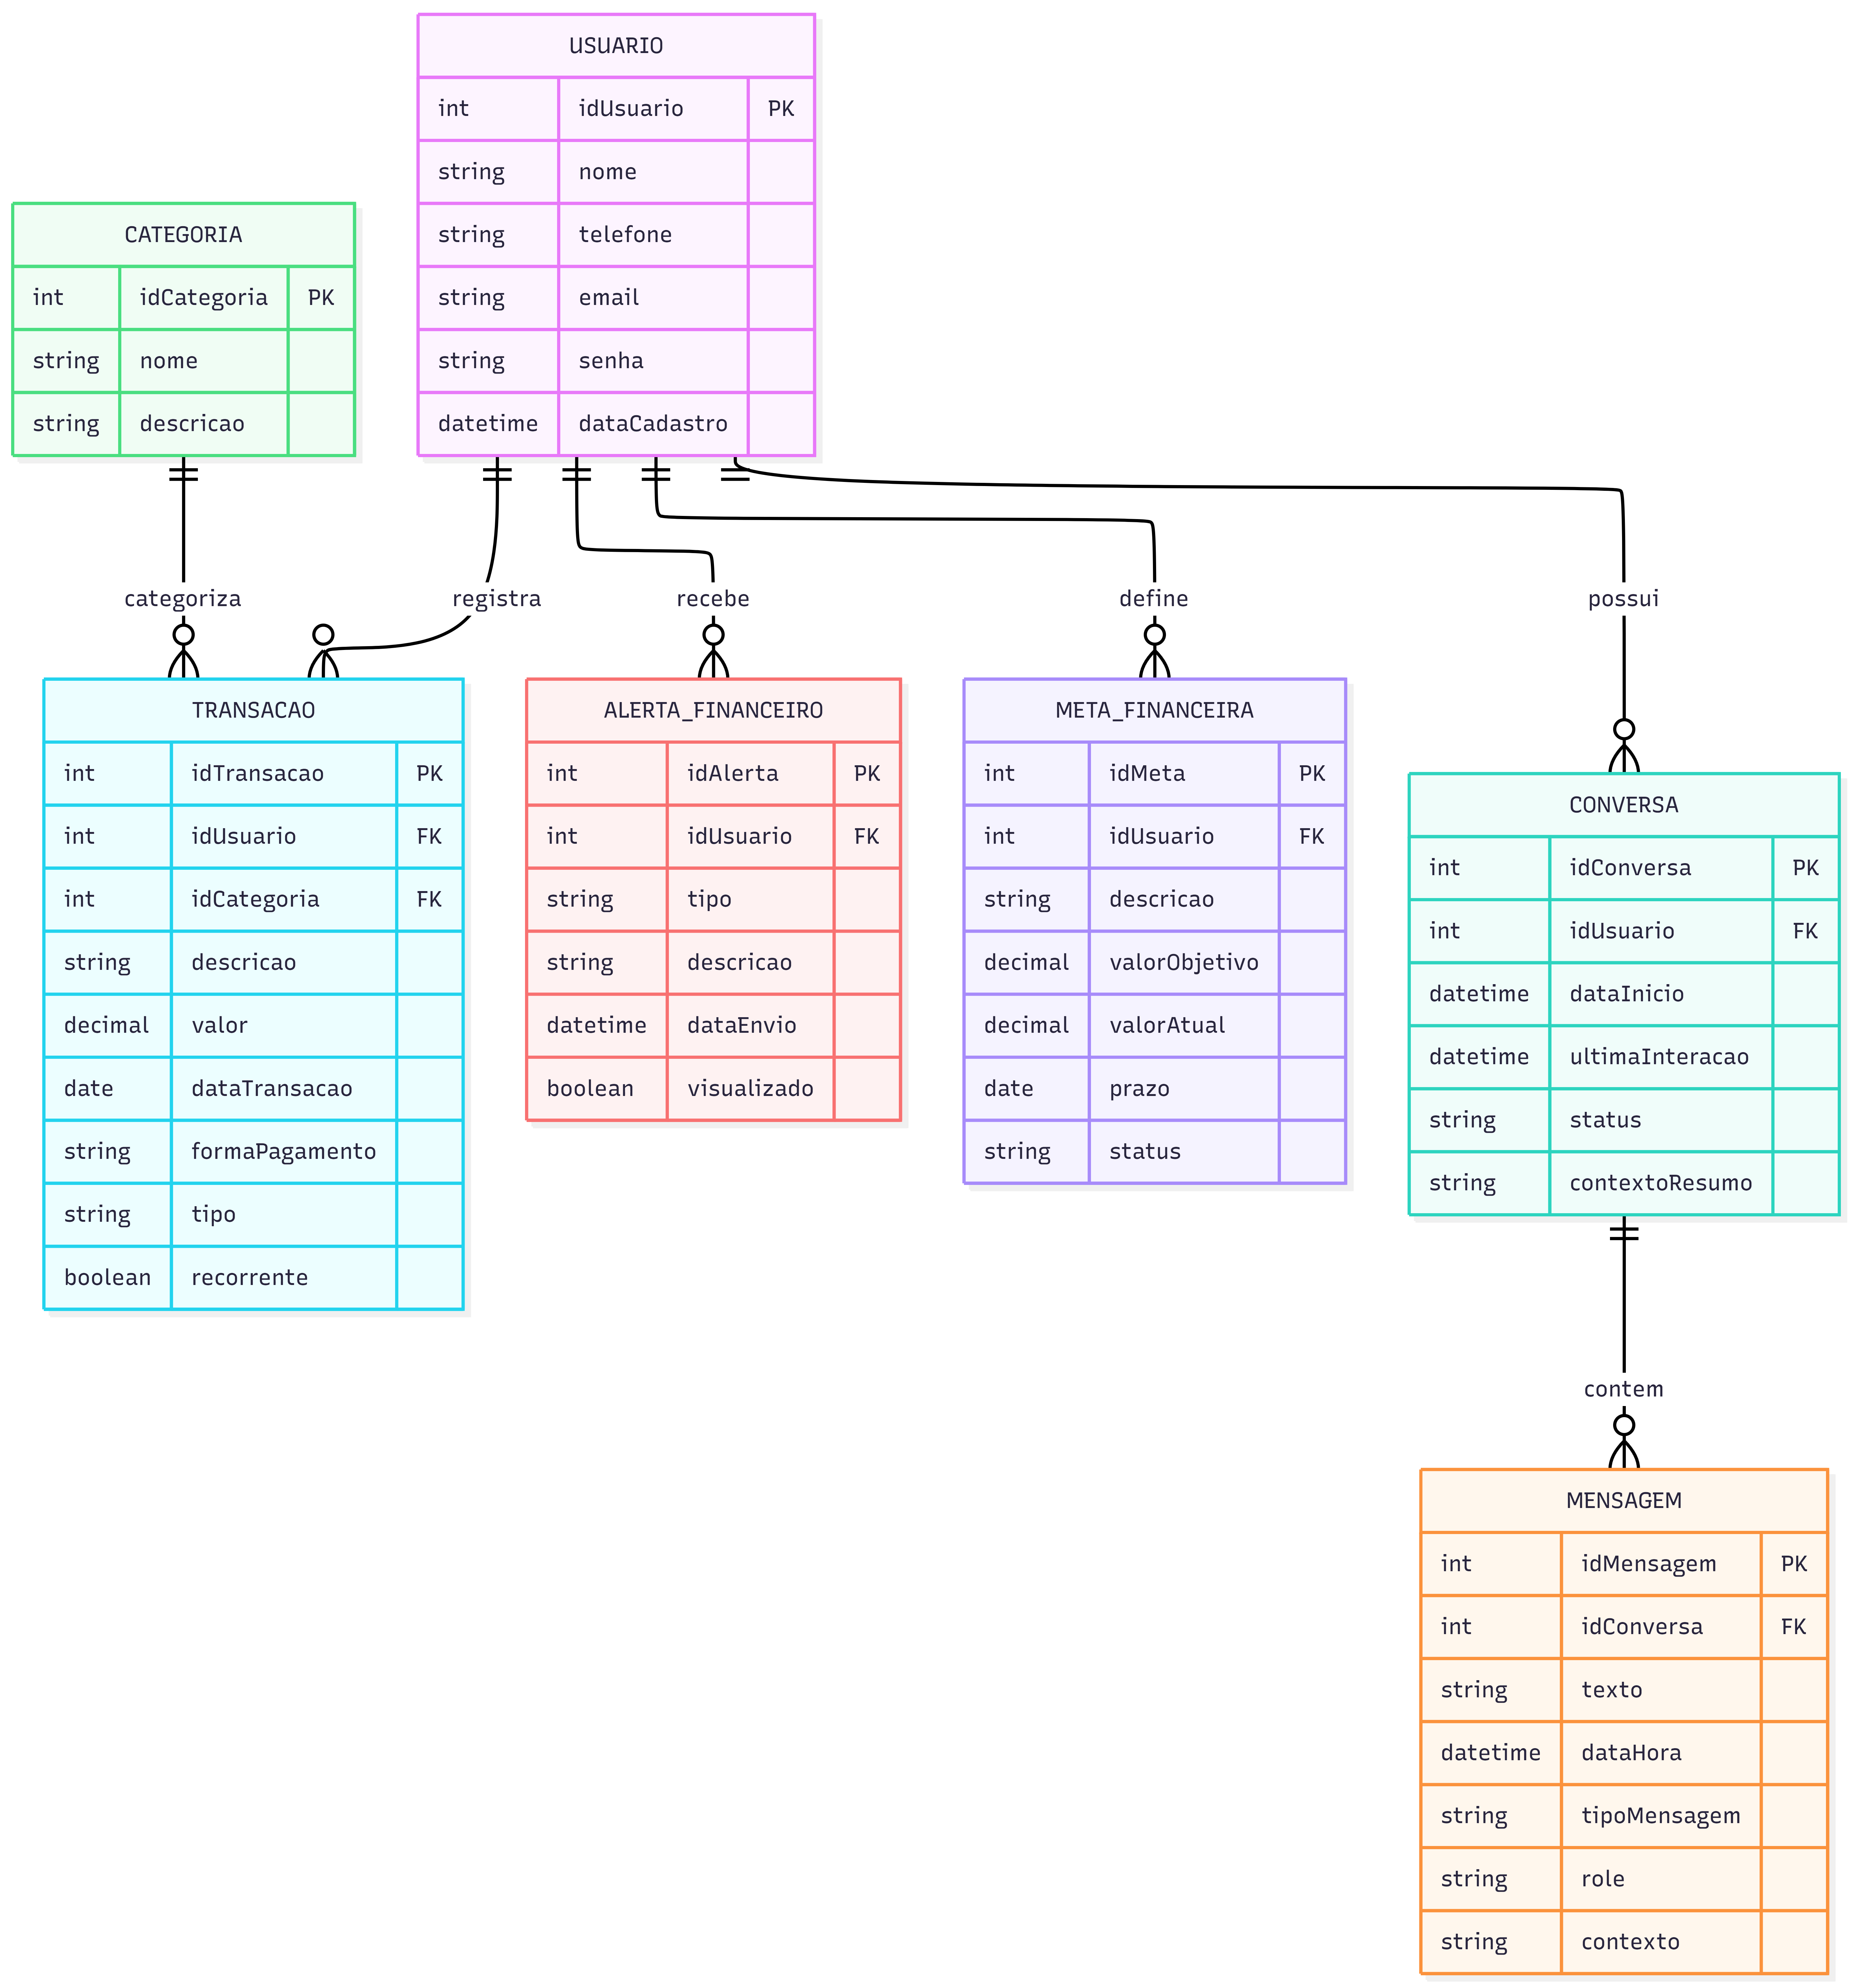
\includegraphics[width=0.8\textwidth]{figs/diagrama-entidade-relacionamento.png}
    \fonte{Elaborado pelos autores.}
\end{figure}

\subsection{Protótipo da Interface de Usuário}

O protótipo da solução contempla dois eixos principais: a experiência conversacional no WhatsApp e a interface web para visualização de dashboards e relatórios. A proposta busca oferecer uma jornada de usuário fluida, começando pelo registro simplificado de gastos via linguagem natural e culminando em uma análise visual completa da saúde financeira.

\subsubsection{Fluxo de cadastro e uso do sistema}

O uso da solução proposta pode começar por dois caminhos. No primeiro, o usuário acessa diretamente a versão web do GranaAI, abre a tela de cadastro e preenche as informações solicitadas pelo sistema. Após a conclusão do formulário, a plataforma confirma o cadastro e permite que o usuário siga para o uso da aplicação.

No segundo caminho, o primeiro contato acontece pelo WhatsApp. Caso o usuário envie uma mensagem ao chatbot antes de possuir cadastro, o sistema identifica que aquele número ainda não está vinculado a nenhuma conta. Em seguida, o assistente informa a necessidade de cadastro e envia o link da tela correspondente.

Depois que o cadastro é finalizado, o usuário recebe uma confirmação na versão web e pode retornar à conversa com o chatbot. A partir desse momento, quando ele enviar uma mensagem relacionada a uma movimentação financeira, como uma despesa ou receita, o sistema associa automaticamente o número de telefone à conta cadastrada.

Com essa vinculação, as informações enviadas pelo WhatsApp passam a ser registradas na base de dados do usuário. Assim, uma mensagem como ``gastei R\$ 35,00 com lanche'' pode ser interpretada pelo chatbot, classificada como despesa e armazenada na categoria correspondente.

Para consultar essas informações na versão web, o usuário acessa a tela de login e informa os dados definidos no cadastro. Após a autenticação, ele visualiza suas movimentações, gráficos, metas financeiras e relatórios gerados a partir dos registros feitos pelo WhatsApp.

\begin{figure}[H]
    \centering
    \caption{Diagrama de sequência de cadastro e registro financeiro}
    \label{fig:diagrama-sequencia-cadastro-registro}
    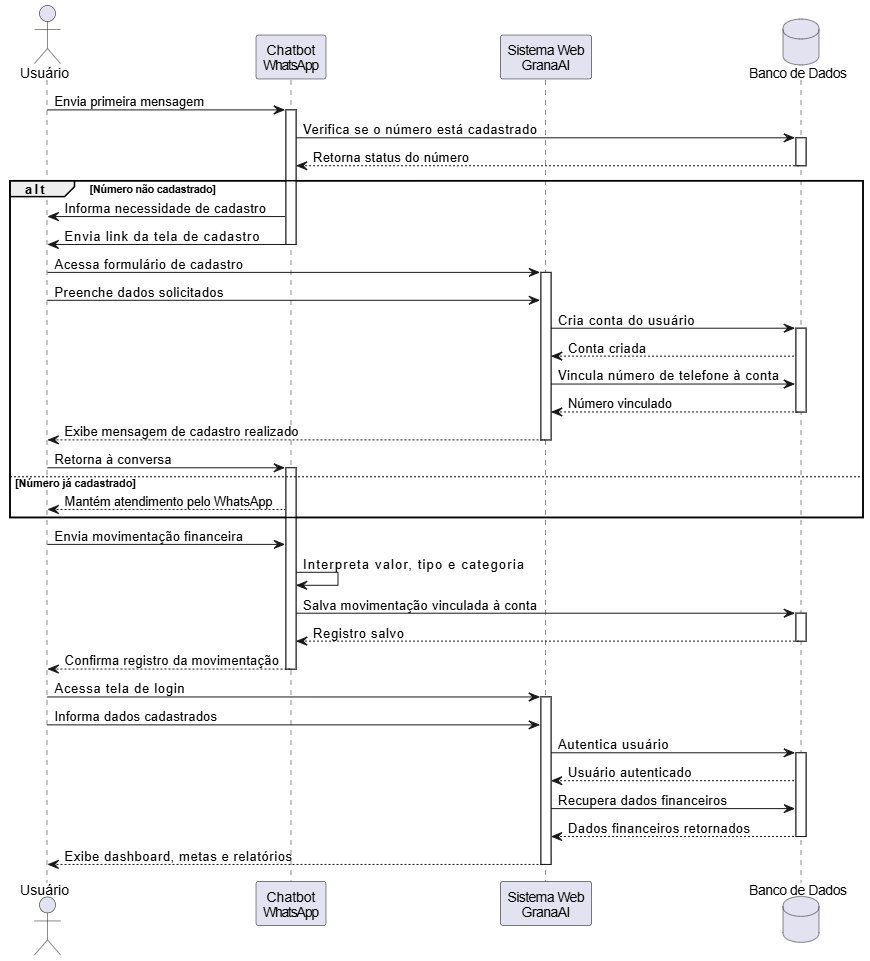
\includegraphics[width=\textwidth]{figs/diagrama-sequencia.png}
    \fonte{Elaborado pelos autores.}
\end{figure}

\subsubsection{Interface Conversacional (WhatsApp)}

A interação no WhatsApp foi projetada para ser rápida e intuitiva. O usuário pode enviar mensagens de texto ou áudio descrevendo um gasto, e o assistente GranaAI processa a informação em tempo real. A Figura \ref{fig:prototipo-whatsapp} ilustra uma simulação de uso onde o usuário registra uma compra impulsiva no iFood. Além de confirmar o registro, a IA fornece um \textit{insight} imediato sobre o limite da categoria, cumprindo o papel de assistente preventivo.

\begin{figure}[H]
    \centering
    \caption{Simulação de registro de gasto via WhatsApp}
    \label{fig:prototipo-whatsapp}
    
\includegraphics[width=0.5\textwidth]{figs/simulado-whatsapp.png}
    \fonte{Elaborado pelos autores.}
\end{figure}

\subsubsection{Dashboard Web}

A interface web serve como o centro de análise financeira do usuário. Nela, os dados registrados via WhatsApp são consolidados em visualizações gráficas que facilitam a compreensão do orçamento. A Figura \ref{fig:prototipo-dashboard} apresenta a visão geral do dashboard, com cartões de resumo financeiro, gráficos de evolução mensal e a lista de transações recentes.

\begin{figure}[H]
    \centering
    \caption{Interface principal do Dashboard Web}
    \label{fig:prototipo-dashboard}
    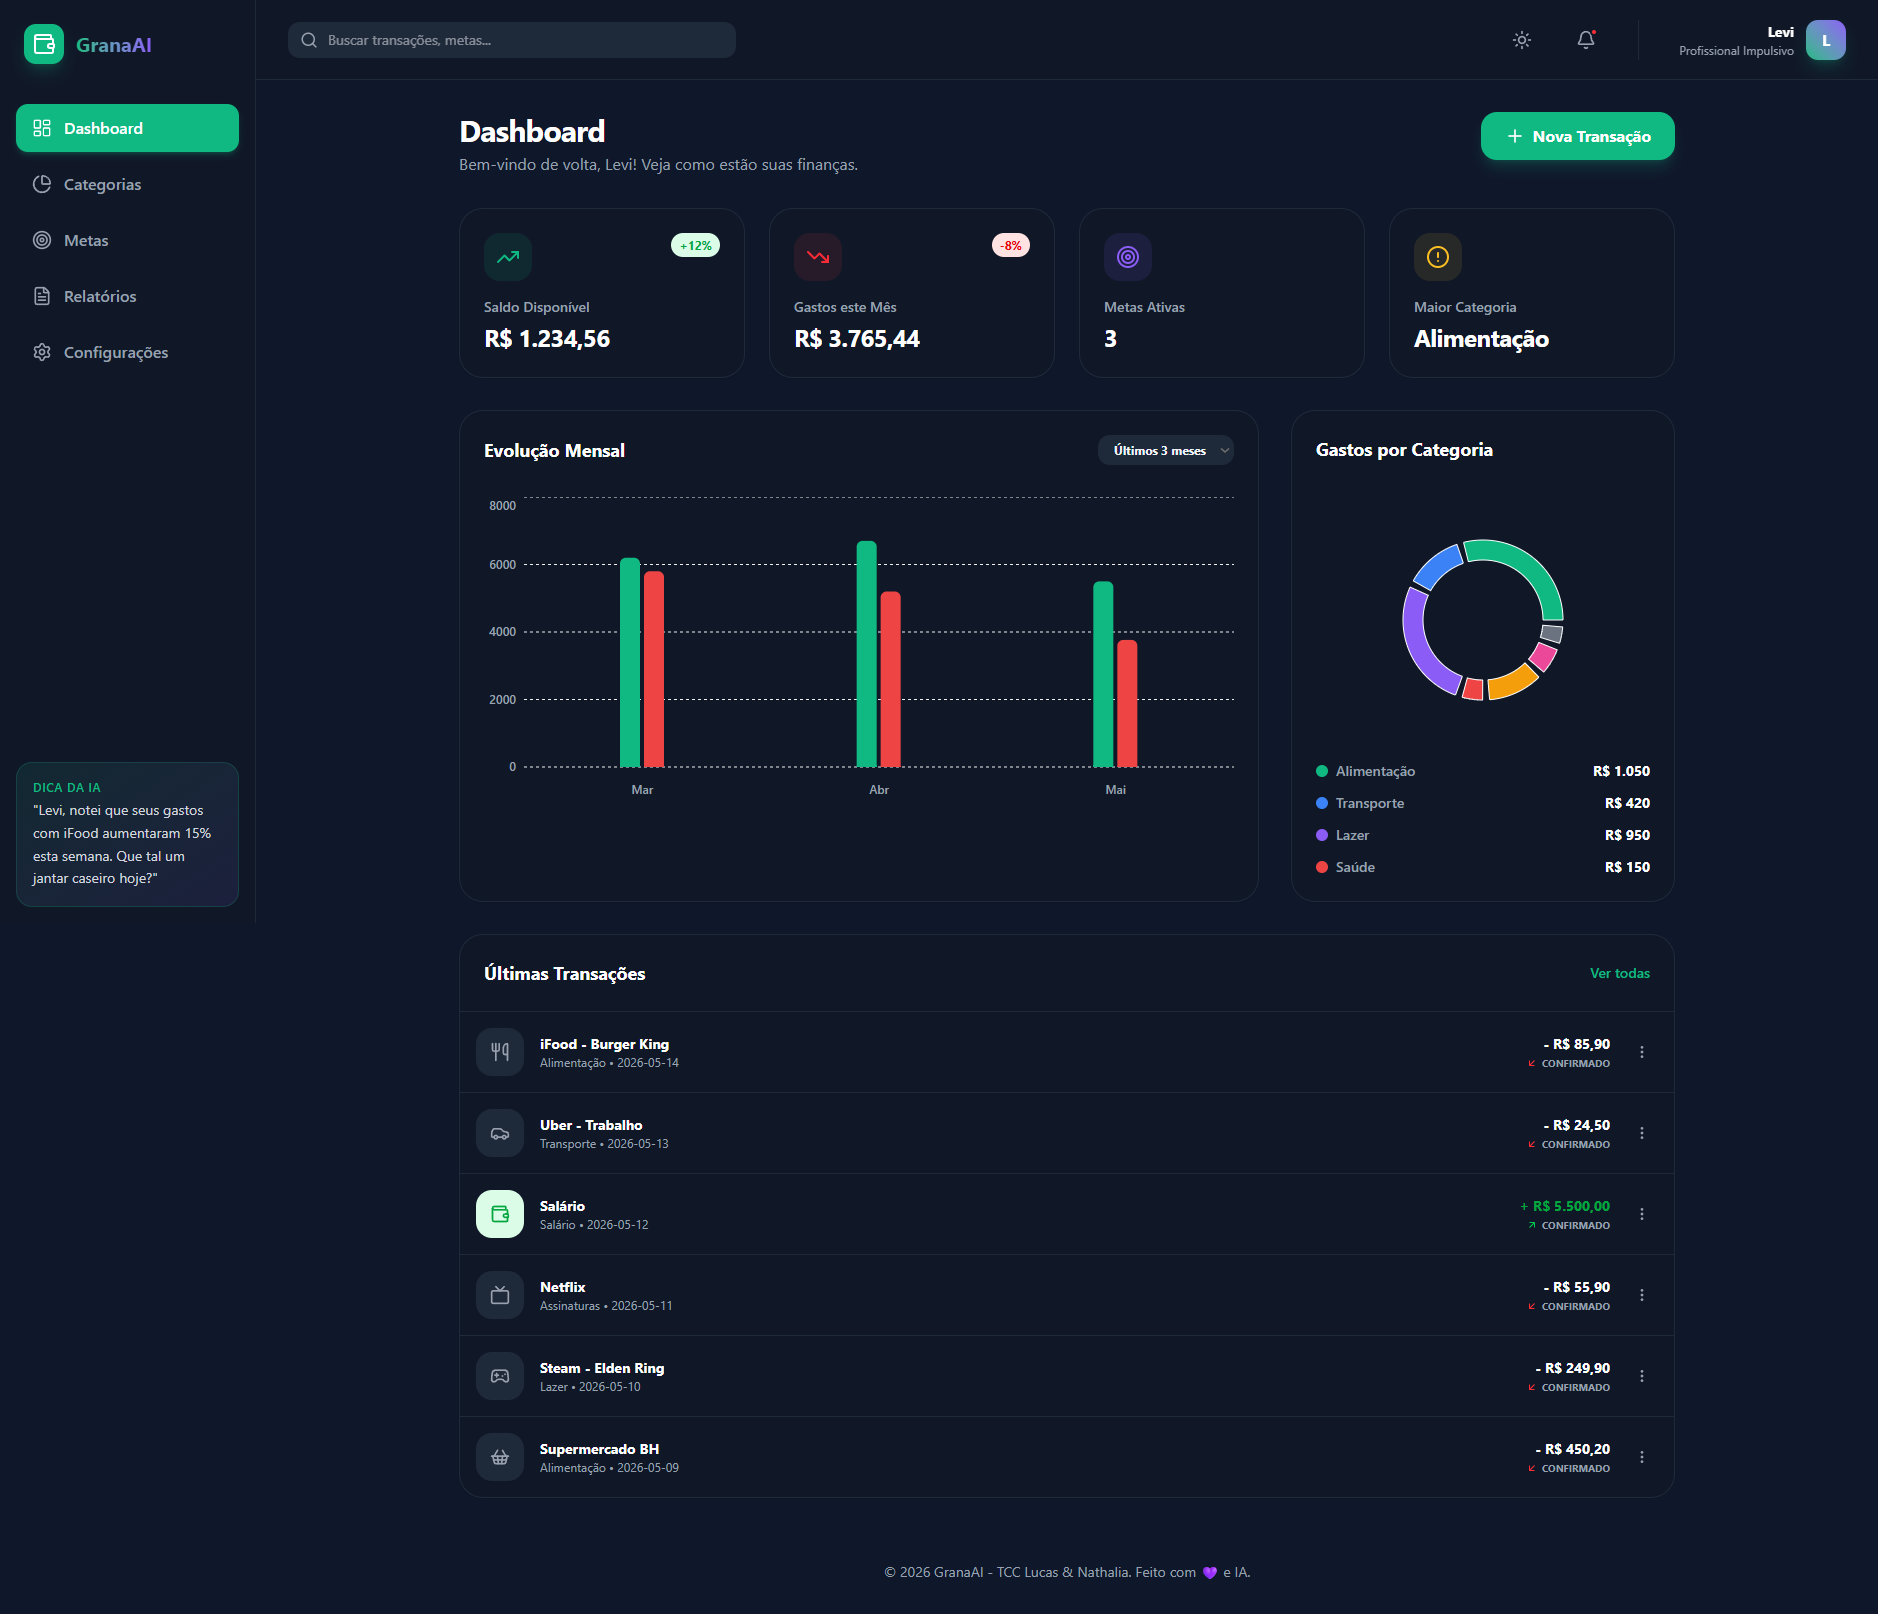
\includegraphics[width=\textwidth]{figs/dashboards.png}
    \fonte{Elaborado pelos autores.}
\end{figure}

As demais funcionalidades, como o gerenciamento de categorias (Figura \ref{fig:prototipo-categorias}) e o acompanhamento de metas financeiras (Figura \ref{fig:prototipo-metas}), complementam a experiência, permitindo que o usuário tenha controle total sobre seus objetivos de médio e longo prazo.

\begin{figure}[H]
    \centering
    \caption{Gerenciamento de limites por categoria}
    \label{fig:prototipo-categorias}
    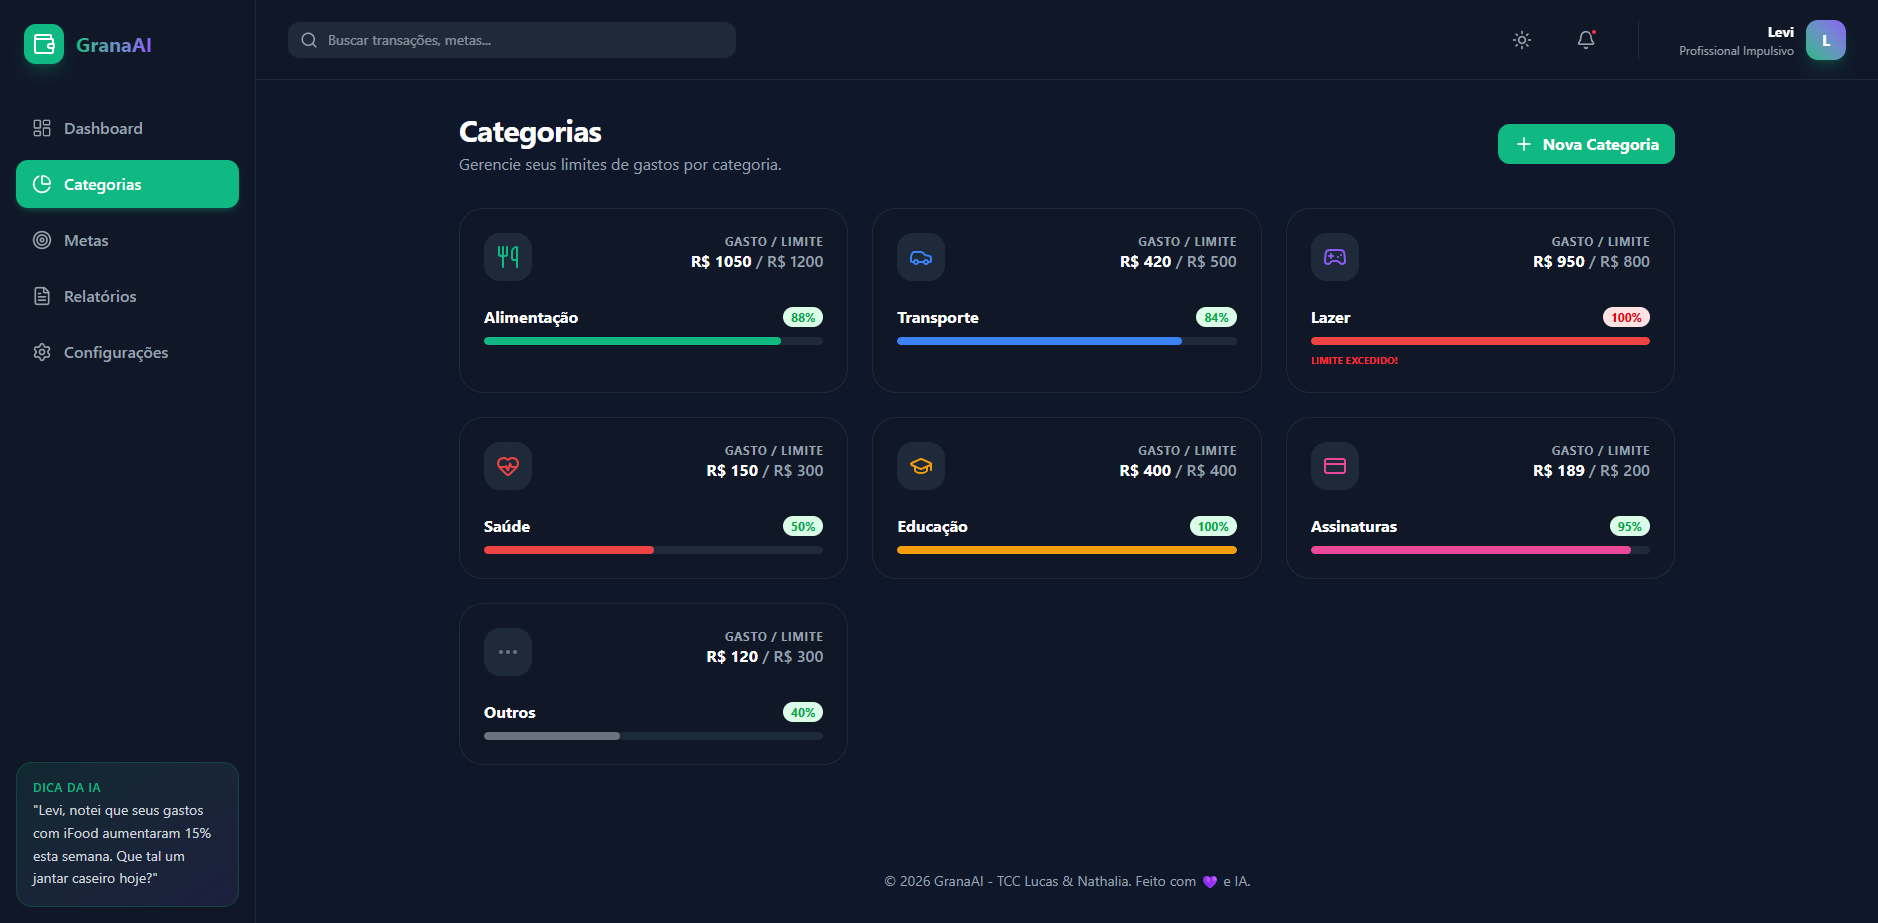
\includegraphics[width=0.8\textwidth]{figs/categorias.png}
    \fonte{Elaborado pelos autores.}
\end{figure}

\begin{figure}[H]
    \centering
    \caption{Acompanhamento de metas financeiras}
    \label{fig:prototipo-metas}
    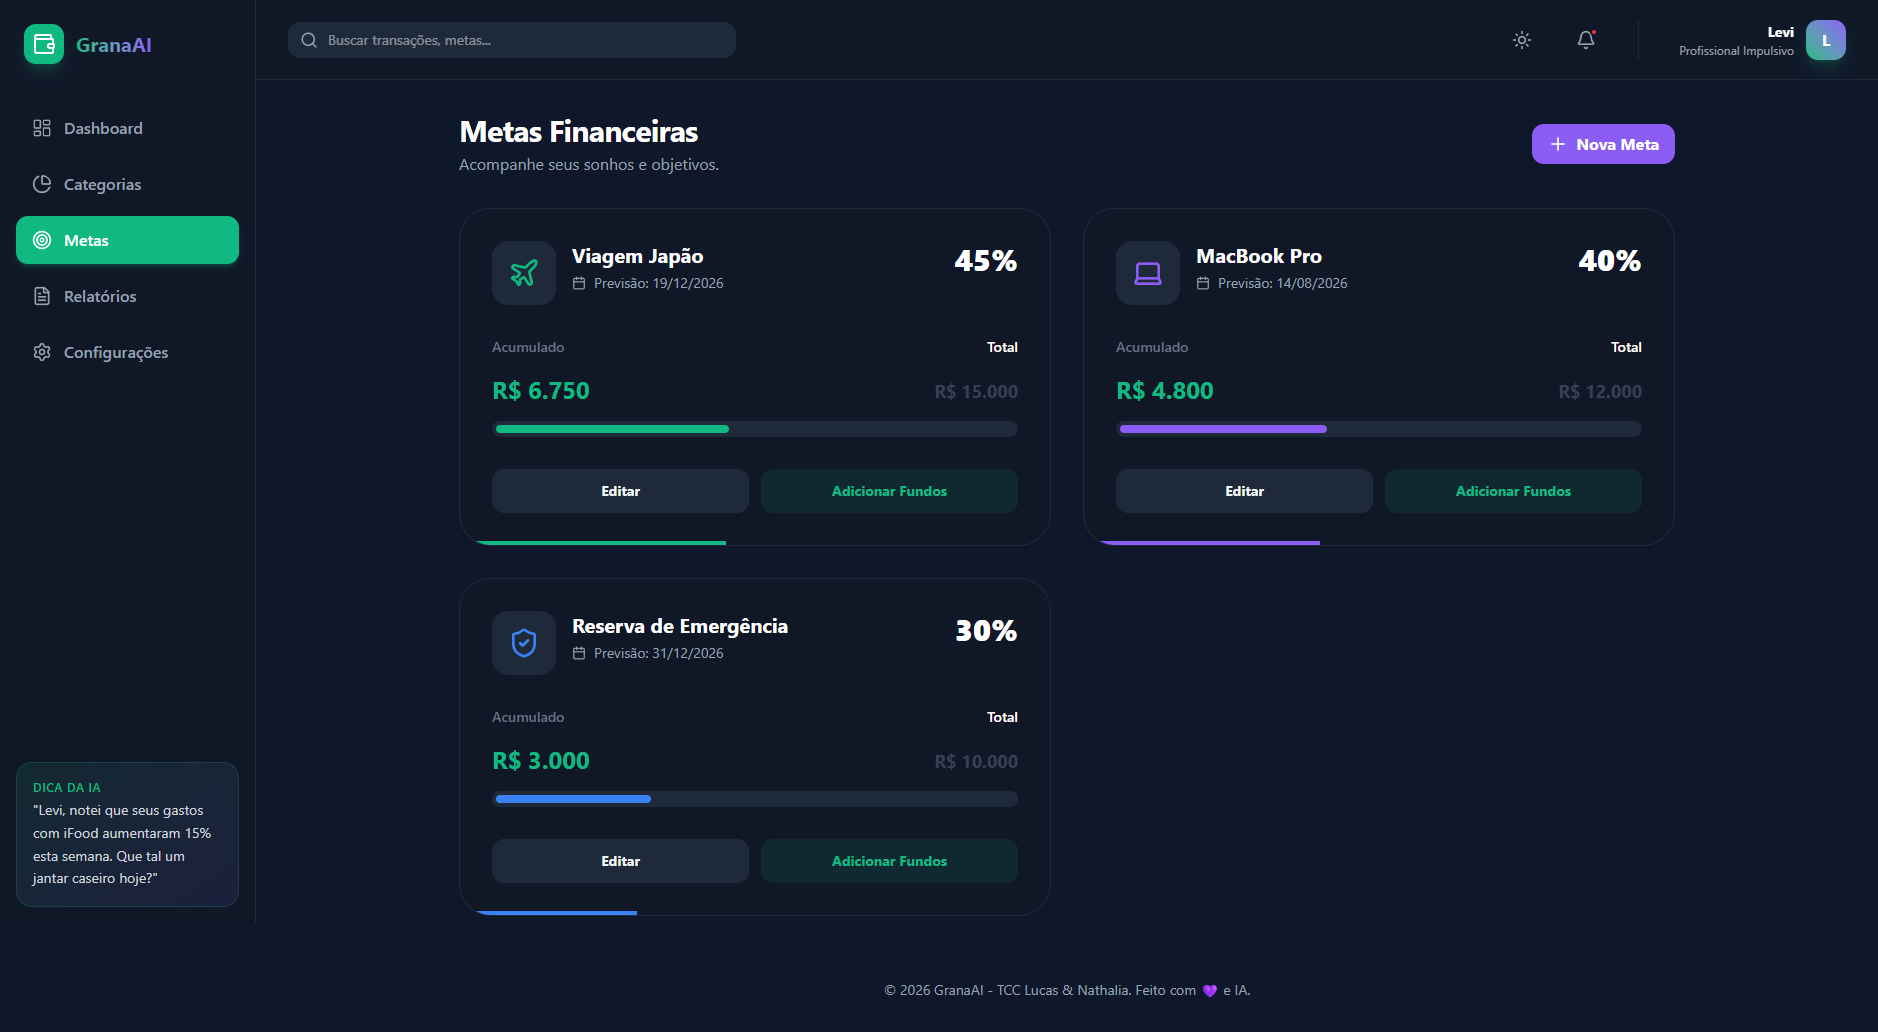
\includegraphics[width=0.8\textwidth]{figs/metas.png}
    \fonte{Elaborado pelos autores.}
\end{figure}

Por fim, a tela de relatórios e \textit{insights} (Figura \ref{fig:prototipo-relatorios}) oferece uma visão analítica e projeções futuras geradas pela IA, auxiliando na tomada de decisão estratégica do usuário.

\begin{figure}[H]
    \centering
    \caption{Relatórios detalhados e insights da IA}
    \label{fig:prototipo-relatorios}
    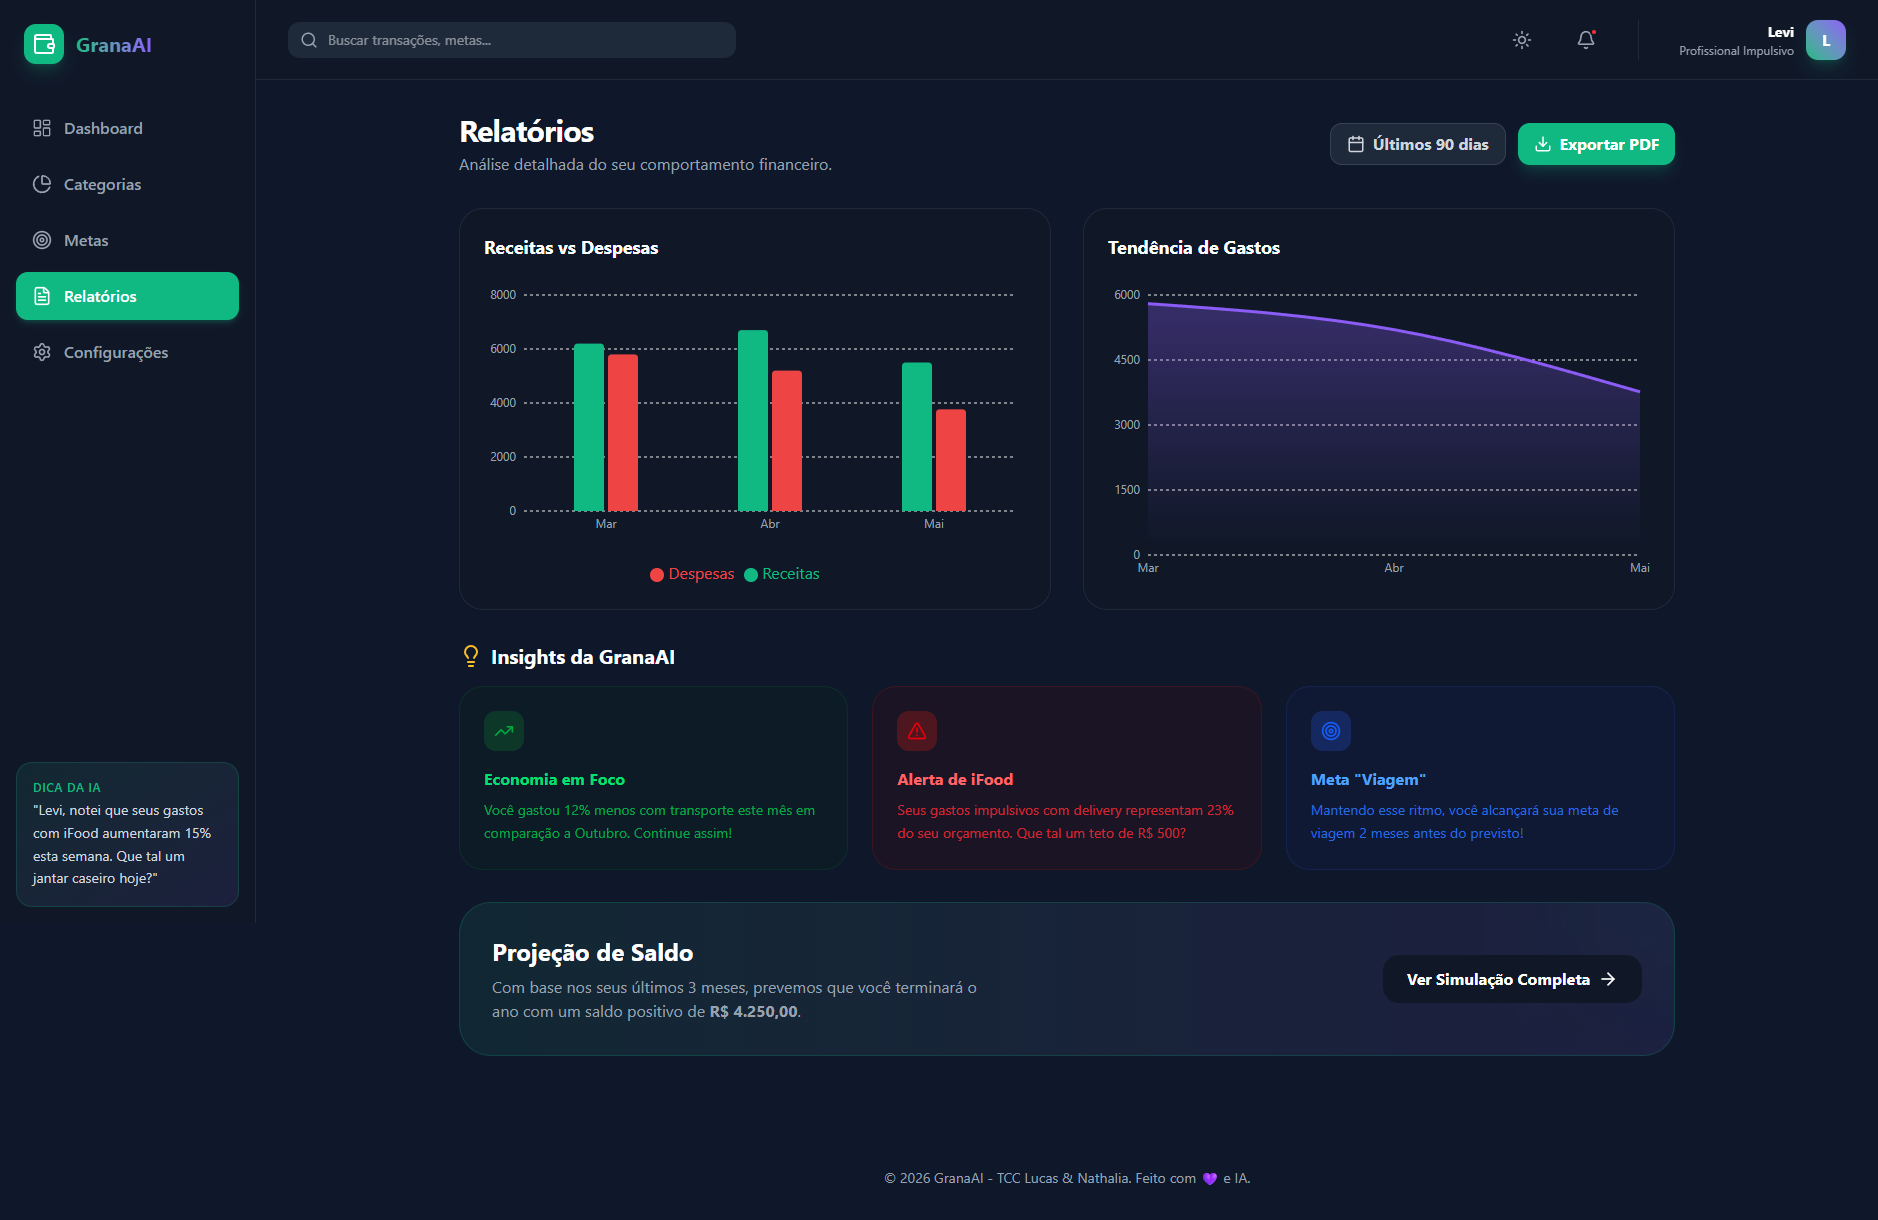
\includegraphics[width=\textwidth]{figs/relatorios.png}
    \fonte{Elaborado pelos autores.}
\end{figure}
